\chapter{Internal Specification}
\label{chap:internal-specifications}

This chapter provides a detailed overview of the application's internal workings. It covers the system's concept, architecture, data structures, components, algorithms, design patterns, and relevant UML diagrams.

\section{System Architecture}

The project's architecture follows the modern Model-View-ViewModel (MVVM) pattern, adhering to Clean Architecture principles. This separation of concerns allows for better maintainability and testability of the code.

\begin{figure}[ht!]
    \centering
    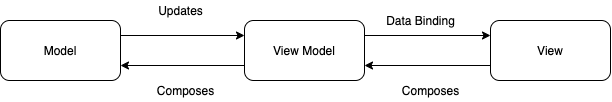
\includegraphics[width=0.7\textwidth]{img/mvvm_explanation.png}
    \caption{High Level MVVM Architecture.}
    \label{fig:mvvm_explanation}
\end{figure}

As shown in Figure ~\ref{fig:mvvm_explanation}, the application is structured into several layers \cite{bib:mvvm}:

\begin{itemize}
    \item \textbf{Application Layer}: Contains the main application logic and navigation.
    \item \textbf{UI Layer}: Responsible for the user interface components, including screens and themes. This layer corresponds to the "View" component of the MVVM pattern.
    \item \textbf{ViewModel Layer}: Manages the data and business logic, providing a bridge between the UI and the Model. This layer corresponds to the "ViewModel" component of the MVVM pattern.
    \item \textbf{Manager Layer}: Handles specific game logic and state management. This layer sits below the view model, and contains the logic for manipulating the models.
    \item \textbf{Repository Layer}: Manages data access and interactions with external sources. This layer is the gatekeeper for the model layer, accessing and manipulating the models before passing it to the application layer.
    \item \textbf{Model Layer}: Represents the data and domain logic of the application. This layer contains the data entities and business rules. This layer corresponds to the "Model" component of the MVVM pattern.
\end{itemize}


\section{Methodology of Design and Implementation}

The design and implementation of the dice game application follow an iterative and incremental development methodology. This approach involves:
\begin{enumerate}
    \item \textbf{Requirement}: Identifying and documenting functional and non-functional requirements.
    \item \textbf{Design}: Creating architectural and component designs, including UML diagrams to visualize system interactions.
    \item \textbf{Implementation}: Developing the application in iterative cycles, focusing on one feature or component at a time.
    \item \textbf{Testing}: Conducting unit, integration, and user acceptance testing to ensure the system meets requirements using JUnit.
    \item \textbf{Documentation}: Documentation of the implemented features and future development possibilities.
\end{enumerate}

\begin{figure}[ht!]
    \centering
    \begin{subfigure}[b]{0.48\textwidth}
        \centering
        
\includegraphics[scale=0.45]{img/play.png}
        \caption{Design Page 1}
        \label{fig:figma_design1}
    \end{subfigure}
    \hspace{0.02\textwidth}
    \begin{subfigure}[b]{0.48\textwidth}
        \centering
        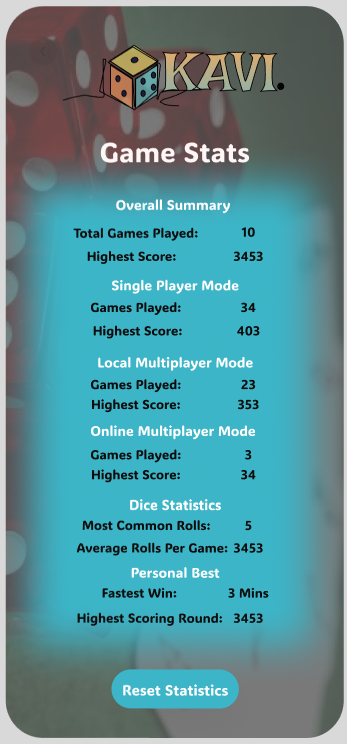
\includegraphics[scale=0.45]{img/stats.png}
        \caption{Design page 2}
        \label{fig:figma_design2}
    \end{subfigure}
    \caption{Initial UI designs and prototypes created in Figma}
    \label{fig:figma_designs}
\end{figure}

\subsection{Design Process}
The application's design process began with creating detailed wireframes and prototypes in Figma. The designs underwent several iterations based on user feedback and technical constraints, evolving into the final implementation. Figure~\ref{fig:figma_designs} shows some of the initial design concepts and their evolution~\cite{bib:kavifigma}.

Various existing solutions and design tools inspired the design of the application, one of which stood out was the board screen design was inspired by a dice application project by binaryshrey~\cite{bib:binaryshrey}. This repository provided a minimalistic and intuitive approach to dice roll applications, which influenced the layout and functionality of the board screen in this project.

\subsection{Model Training}

The dice detection model was developed using Roboflow's platform, which streamlined the entire process from dataset creation to deployment. The training dataset, shown in Figure~\ref{fig:roboflow_dataset}, consisted of carefully annotated dice images across various conditions, ensuring robust detection performance in real-world scenarios.

\begin{figure}[ht!]
    \centering
    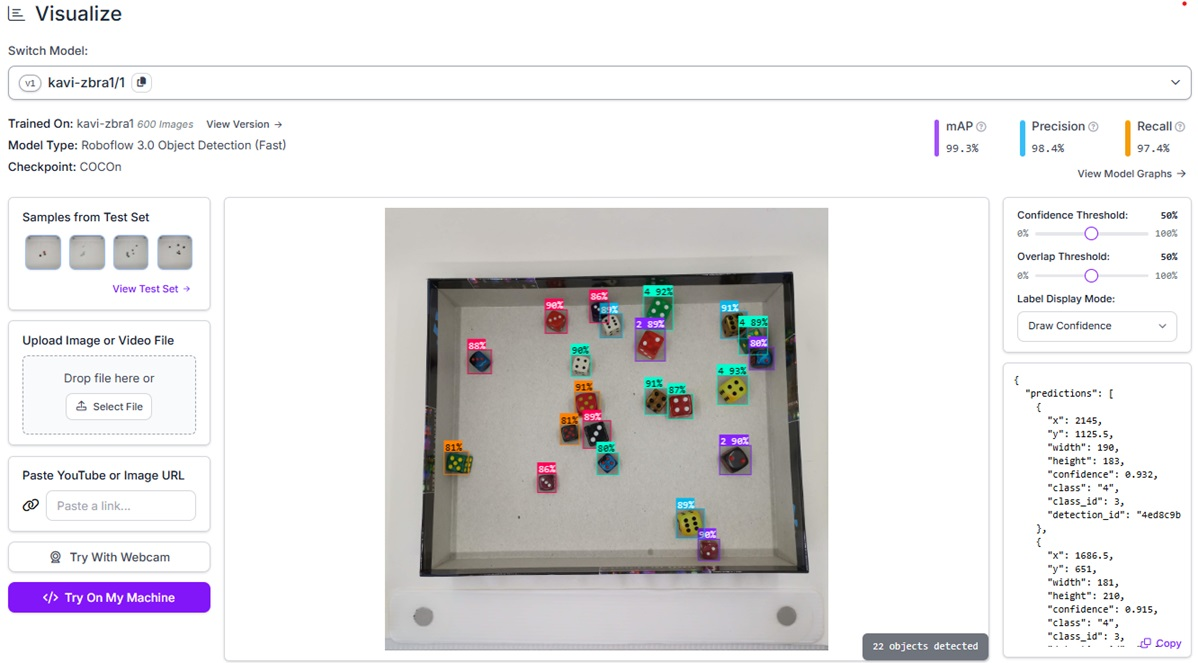
\includegraphics[width=\textwidth]{img/roboflow_dataset.jpg}
    \caption{Roboflow dataset management interface showing dice image annotations}
    \label{fig:roboflow_dataset}
\end{figure}

Roboflow facilitated data augmentation and preprocessing, which enhanced the dataset's diversity. The model training and optimization phases were crucial for achieving high accuracy, while the deployment and API integration ensured seamless real-time inference capabilities.

\subsection{Project Timeline}

The project was implemented following a structured timeline as shown in Figure ~\ref{fig:gantt}. The development process was organized into major phases, including planning, design, core development, AI integration, and testing, with regular milestones to track progress.

\begin{figure}[ht!]
    \centering
    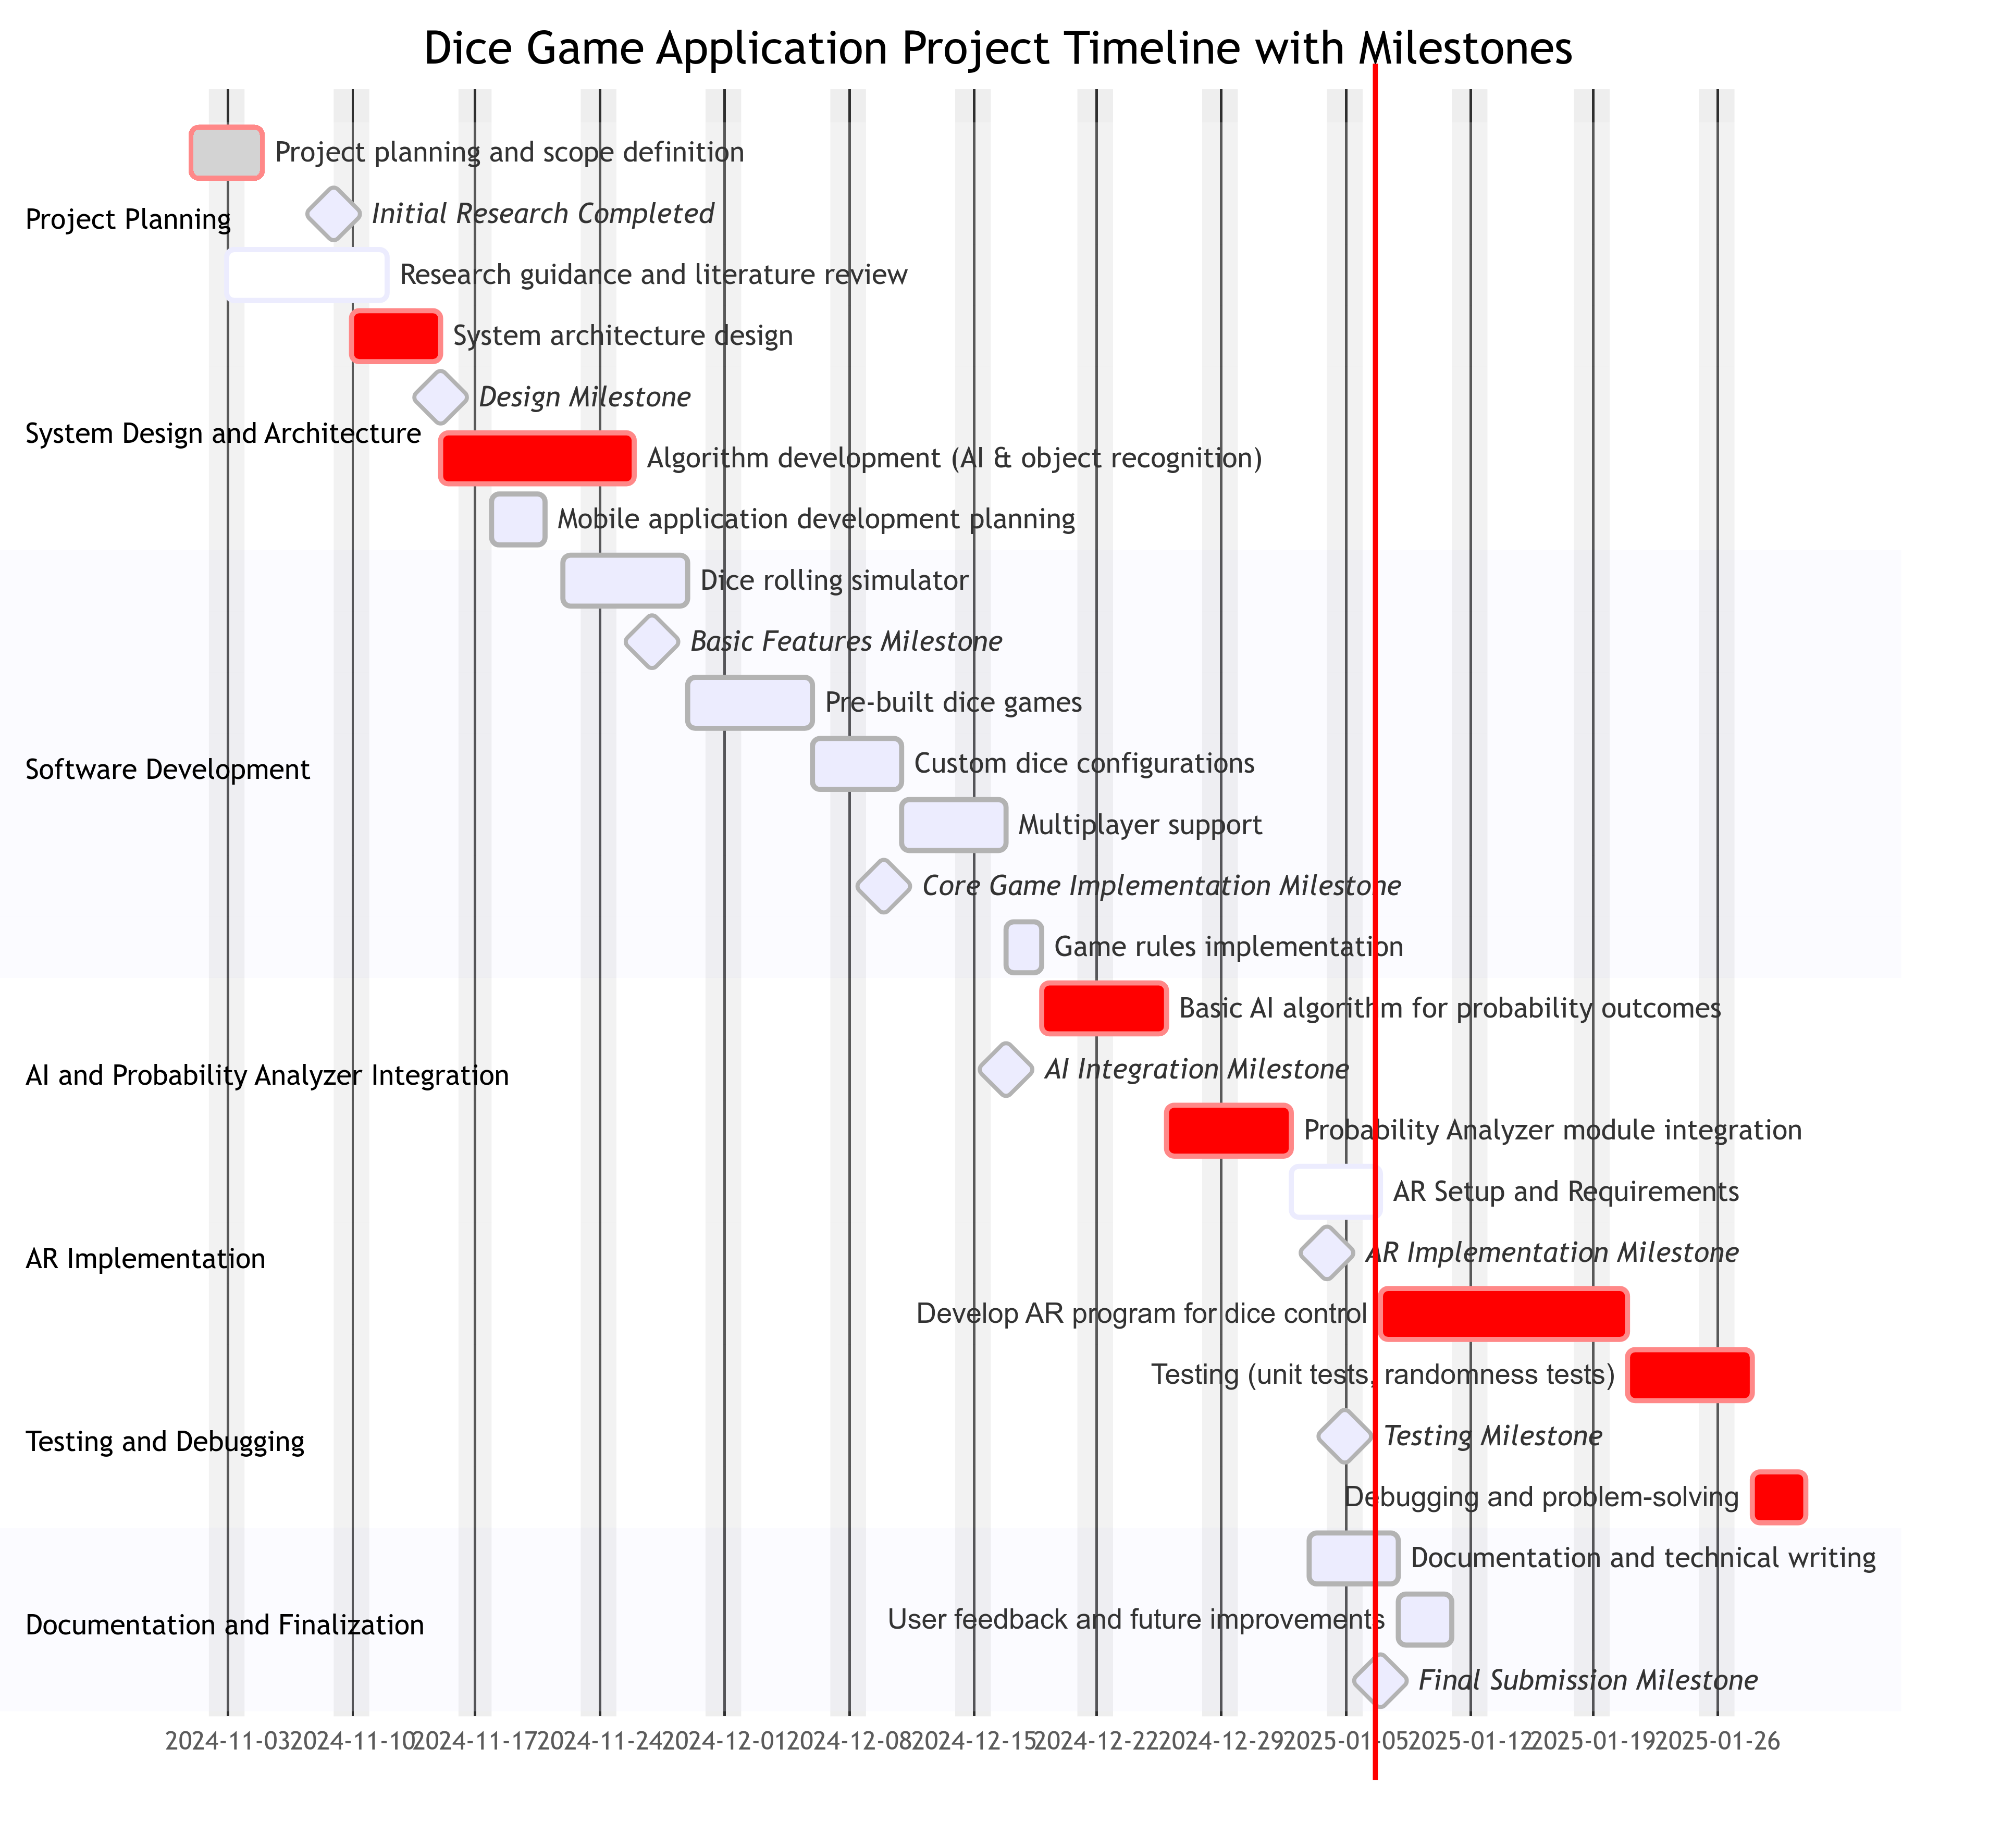
\includegraphics[width=\textwidth]{img/gantt_chart.png}
    \caption{Project Gantt chart showing development phases and milestones}
    \label{fig:gantt}
\end{figure}

This structured approach allowed for continuous improvement and adaptation to changing requirements, ensuring a high-quality application. While some initially planned features like AR implementation were identified as future enhancements, the focus remained on delivering a robust core game experience with AI capabilities.

\section{Data Structures and Data Management}

The application utilizes a variety of data structures to effectively manage game state, user profiles, and game data. These structures are designed for efficiency and scalability, supporting the diverse features of the game. Data persistence is achieved using DataStore, a modern data storage solution, and dependency injection is managed using Dagger Hilt.

\subsection{Data Models}

The application's data is represented using models located in the `models` directory. These models encompass different aspects of the game, including game state, user data, and results from the image detection mechanisms.

\subsubsection{Game Models}

The core game models are:
\begin{itemize}
    \item \textbf{GameStatistics}: Tracks overall game performance metrics for each user across all games. These metrics include total games played, win rates, average scores, and other relevant data.
    \item \textbf{GameScoreState}: Holds the current score and state of the game during an individual game session, including the score for each player and the game's current turn.
     \item \textbf{DecisionPatterns}: Captures the different decision-making patterns of a player in each game, including when the player decides to hold dice, or when they decide to roll or bank scores. This is used to calculate statistics about how players are playing the game.
    \item \textbf{WinRate}: Calculates and stores the win rate of a player. This will be used in \textit{PlayerAnalysis}.
    \item \textbf{TimeMetrics}: Stores metrics about how long a player played the game, including the amount of time a player has spent playing each game, and the time spent per round. This is used in \textit{PlayerAnalysis}.
    \item \textbf{PlayerAnalysis}: Provides detailed analysis of a player's behavior and performance trends, combining data from various sources like `WinRate`, `TimeMetrics`, and `DecisionPatterns`. It tracks trends over time, identify strong and weak areas of a player, and provides an overall evaluation of a player's performance.
\end{itemize}

\subsubsection{Detection Models}

The detection models, located in the `detection` subdirectory of `models`, are:

\begin{itemize}
    \item \textbf{DiceDetectionResult}: Captures results from dice detection processes, including the number detected and the number on each die.
    \item \textbf{Detection}: Represents the state of the detection model.
    \item \textbf{DetectionRequest}: Represents the request to start the detection.
    \item \textbf{DetectionResponse}: Represents the response from the detection.
    \item \textbf{ImageInfo}: Holds the information of the image used for detection.
    \item \textbf{Prediction}: Represents a single prediction from the detection model.
\end{itemize}

\subsection{Data Management}

The application uses a modern and efficient approach to data management, leveraging DataStore for persistent storage and Dagger Hilt for dependency injection.

\subsubsection{Persistent Storage}

DataStore provides a robust, asynchronous solution for managing the application's persistent data. Unlike traditional databases, DataStore offers type safety and a reactive approach, ensuring smooth and efficient data handling for user preferences, game statistics, and other relevant application data. This approach helps the application to provide quick access to stored data and avoids some of the limitations of other persistent storage options.

\subsubsection{Dependency Injection}
Dagger Hilt simplifies the management of dependencies by providing a standardized way to inject components into the application. This improves code modularity, making the app easier to test, maintain, and scale. Dagger Hilt helps manage the dependencies between classes and is used to ensure all modules are configured correctly, and this creates a more efficient way to manage the dependencies of the application, while also making testing easier.

\section{Components, Modules, and Classes}

This section outlines the core components, modules, and classes that form the foundation of the application. It provides a summary of essential classes, detailing their roles and responsibilities.

\subsection{Application Classes}
The main classes of the application can be categorized into Main Application Classes, ViewModels, and Managers.
\subsubsection{Main Application Classes}
\begin{itemize}
    \item \textbf{KaviApplication}: The main class that extends Android's Application class, responsible for initializing the application, and important libraries like Timber for debugging.
    \item \textbf{MainActivity}: The main entry point for the application, sets up the primary UI, and manages navigation.
\end{itemize}

\subsubsection{ViewModels}
\begin{itemize}
  \item \textbf{AppViewModel}: Manages application-wide data and state, coordinating between different parts of the application.
    \item \textbf{GameViewModel}: Manages data and logic specific to each game, providing a bridge between the view and the data and state.
      \item \textbf{DetectionViewModel}: Manages the state and logic of the image detection process, and exposes this data to the UI layer.
\end{itemize}

\subsubsection{Managers}
\begin{itemize}
    \item \textbf{MyGameManager}: Handles the state management and the logic of the custom game board.
    \item \textbf{PigGameManager}: Manages the game state, rules, and scoring for the Pig game.
     \item \textbf{GreedGameManager}: Manages the game state, rules, and scoring for the Greed game.
    \item \textbf{BalutGameManager}: Manages the game state, rules, and scoring for the Balut game.
     \item \textbf{DiceManager}: Manages the various aspects of rolling the dice, and its state.
    \item \textbf{DataStoreManager}: Manages the saving and retrieval of data from the DataStore.
     \item \textbf{StatisticsManager}: Manages the collection and processing of game statistics.
    \item \textbf{SettingsManager}: Manages the saving and loading of the application's settings.
     \item \textbf{ShakeDetectorManager}: Manages the logic of the shake gesture.
\end{itemize}

\vspace{0.2cm}
A detailed Class diagram is included in the UML diagram provided in section ~\ref{sec:uml}.

\section{Algorithms and Implementations}

The application implements several sophisticated algorithms to provide an engaging and intelligent gaming experience. 

\subsection{Image Processing Pipeline}

The dice recognition system uses a sequence of image processing steps implemented in `RoboflowRepositoryImpl`, a class responsible for handling communication with the Roboflow API:
\subsubsection{Preprocessing}
    \begin{itemize}
        \item RGB conversion using `ensureRGBFormat()` to guarantee that the image is in the correct format for processing.
        \item Contrast enhancement through `enhanceContrast()` using histogram-based normalization to make the dice pips more clear.
        \item Aspect ratio scaling via `scaleWithAspectRatio()` to make sure that the images are of the correct size.
        \item Noise reduction with `reduceNoise()` to reduce the noise in the image.
    \end{itemize}
\subsubsection{Detection}
    \begin{itemize}
        \item API integration with Roboflow service using the `RoboflowClient`, which makes a call to the Roboflow API and gets the result.
        \item Confidence filtering (threshold: 40\%) which removes detections with less than 40\% confidence to avoid erroneous detections.
        \item Non-maximum suppression, performed by using a library for detection, which removes overlapping bounding boxes, by selecting the bounding boxes with the highest score and removing those that are overlapping.
    \end{itemize}

\subsection{AI Strategy System}

The AI decision-making system, which is responsible for determining the optimal moves for the AI, is implemented across multiple manager classes. The strategy is designed to consider the current game state and make intelligent decisions based on the game variant. Below are the key methods used by the AI to guide its decisions:
    
\begin{itemize}
\item  \textit{`shouldAIBank()`} is responsible for determining when the AI should bank points based on the current turn’s score, its total score, and the player's total score. The decision is dependent on the game variant being played, such as the "Greed" or "Pig" game mode. If the AI is playing a "Greed" or "Pig" game, it assesses whether continuing to roll is risky based on the points accumulated so far. If the risk outweighs the potential gain, the AI decides to bank.
       
\begin{lstlisting}[language=Kotlin,caption={Should AI Bank Function.}, label={lst:shouldAIBank}]
    fun shouldAIBank(currentTurnScore: Int, aiTotalScore: Int, playerTotalScore: Int): Boolean =
        when (_selectedBoard.value) {
            GameBoard.PIG.modeName -> pigGameManager.shouldAIBank(
                currentTurnScore = currentTurnScore,
                aiTotalScore = aiTotalScore,
                playerTotalScore = playerTotalScore
            )
            GameBoard.GREED.modeName -> greedGameManager.shouldAIBank(
                currentTurnScore = currentTurnScore,
                aiTotalScore = aiTotalScore
            )
            else -> false
        }
\end{lstlisting}
    
\item \textit{`chooseAICategory()`} is used to select the optimal scoring categories for the Balut AI based on the dice rolled. The AI evaluates the current dice and determines which scoring category will maximize its chances of winning, such as the best combination of dice values for the current state of the game. If the game state is invalid or not initialized, it will first initialize the Balut game before making a decision.
       
\begin{lstlisting}[language=Kotlin,caption={Choose AI Category Function.}, label={lst:chooseAICategory}]
    fun chooseAICategory(diceResults: List<Int>): String {
        val currentState = (_gameState.value as? GameScoreState.BalutScoreState) ?: run {
            Timber.e("Invalid game state for AI category selection")
            return balutGameManager.initializeGame().let {
                balutGameManager.chooseAICategory(diceResults, it)
            }
        }
        return balutGameManager.chooseAICategory(diceResults, currentState)
    }
    \end{lstlisting}
    
\end{itemize}
    
These methods ensure that the AI can make well-informed decisions based on its current state and the game rules, allowing for a challenging and adaptive opponent in each game variant.
    

\subsection{Statistics System}
The statistics tracking system, which is used for analyzing and processing user data, is centralized in `StatisticsManager`:

\subsubsection{Game Analytics}
    \begin{itemize}
        \item \textit{`updateGameStatistics()`} records game outcomes for the players, and saves it to the `GameStatistics` model.
        \item \textit{`updateTimeMetrics()`} tracks timing data, including the time spent in each round, and the total time spent in a game.
        \item \textit{`updatePerformanceMetrics()`} calculates improvement rates, by keeping track of how many games the player wins, and their high scores.
    \end{itemize}

\subsubsection{Achievement Processing}
The achievement processing is responsible for monitoring and managing user progress toward unlocking achievements in the application. The following key functions are implemented:
    \begin{itemize}
        \item \textit{`calculateAchievements()`}: Evaluates the unlock conditions for all achievements available in the application and updates their status based on the latest user activity and metrics.
        \item \textit{`updateProgressMetrics()`}: Tracks progress toward achievement goals by calculating how close the user is to meeting the requirements for unlocking various achievements.
    \end{itemize}
    
\section{Applied Design Patterns}

This application uses several design patterns to enhance code organization and maintainability:

\begin{itemize}
    \item \textbf{Observer Pattern}: Used in the ViewModel layer with Kotlin Flow (StateFlow) to manage and notify the UI of data changes, ensuring a reactive user interface. This allows the UI to update automatically when the state of the application changes. Examples include dice state updates, game statistics updates, and detection results.
    
    \item \textbf{Singleton Pattern}: Employed for managing shared resources using Dagger Hilt's dependency injection. This avoids the need to manually create singletons. Key singletons include the `StatisticsManager` for collecting and managing game analytics, the `GameTracker` for monitoring gameplay sessions, and the `DataStoreManager` for providing access to persistent storage.

    \item \textbf{Factory Pattern}: Implemented using Dagger Hilt's module system to dynamically provide `GameManager` instances (such as `PigGameManager`, `GreedGameManager`, `BalutGameManager`) based on the selected game mode. This approach abstracts object creation by separating the responsibility of object creation from the main code logic and creating the instances of the game managers on the go, without having to specify which instance to create, promoting flexibility and scalability in managing different game variants.
\end{itemize}

\section{UML Diagrams}
\label{sec:uml}

This section presents the UML diagrams that illustrates the architecture and dynamic interactions within the application.

\subsection{Class Diagram}  
The class diagram (Figure~\ref{fig:class_diagram}) provides a visual representation of the static structure of the application, outlining the main classes, their attributes, methods, and how they interact with one another. Key elements shown in this diagram include game states, player analysis, performance metrics, and detection-related classes that capture the core logic and data flow within the app. For instance, the \texttt{GameState} class tracks the game's progress, while the \texttt{DiceDetectionResult} class manages dice recognition results.

\begin{figure}[ht!]
    \centering
    \includesvg[width=1.0\textwidth]{uml/render/class_diagram.svg}
    \caption{Class Diagram of the Application, showing key classes and their relationships.}
    \label{fig:class_diagram}
\end{figure}

\subsection{Models Diagram}  
Figure~\ref{fig:models_diagram} presents the models diagram, which illustrates the data structure of the application. It shows the relationships between various data models, such as \texttt{GameState}, \texttt{GameStatistics}, and \texttt{Detection}. This diagram helps to understand how data is stored and manipulated across different components of the application. For example, the \texttt{Detection} class stores information about recognized objects in the dice, while the \texttt{GameStatistics} class tracks overall game data.

\begin{figure}[ht!]
    \centering
    \includesvg[width=1.0\textwidth]{uml/render/models_diagram.svg}
    \caption{Models Diagram of the Application, showing the relationships between data models.}
    \label{fig:models_diagram}
\end{figure}

\subsection{Structure Diagram}  
The structure diagram (Figure~\ref{fig:package_structure}) outlines the modular organization of the application's packages, highlighting their dependencies and logical groupings. This diagram provides an overview of the application architecture, which is split into layers like the data layer, UI layer, and utility classes. For example, the \texttt{data} package encompasses models, managers, and repositories, while the \texttt{ui} package contains screens, components, and view models. This diagram helps to visualize the overall design and dependencies between different components of the app.

\begin{figure}[ht!]
    \centering
    \includesvg[width=1.0\textwidth]{uml/render/package_structure.svg}
    \caption{Package Structure of the Application, showing the organization of components and their dependencies.}
    \label{fig:package_structure}
\end{figure}


\section{Sequence Diagrams}

Sequence diagrams are used to show the dynamic interactions between various components and objects within the game. They provide a clear visualization of the message flow and the sequence of operations in key scenarios. In this section, we present sequence diagrams that depict the game flow, virtual mode flow, and analysis flow within the application.

\subsection{Game Flow Sequence}

The game flow sequence shows how different components interact during a typical game session. Figure ~\ref{fig:game_flow} shows the process starting from the player initiating a game to the end of the game.

\begin{figure}[ht!]
    \centering
    \includesvg[width=1.0\textwidth]{uml/render/game_flow.svg}
    \caption{Game Flow Sequence in the Application}
    \label{fig:game_flow}
\end{figure}

The process begins when the player initiates the game through the `GameScreen`. The `GameScreen` then initiates the `GameViewModel`, which starts the game through the `GameManager`, and begins a timer using the `StatisticsManager`, while also setting up a shake detection manager with the `ShakeDetectionManager`. During gameplay, the player will interact with the `GameScreen` to either roll the dice using a shake or a manual roll, toggle the held dice, or bank their score. These user actions are propagated to the `GameViewModel`, which manipulates the different managers accordingly. At the end of the game the results are shown to the player and the statistics are updated through the `StatisticsManager`. The game flow will end if the player exits the game, or if they win.

\subsection{Virtual Mode Sequence}

The virtual mode sequence, shown in Figure ~\ref{fig:virtual_mode_flow}, demonstrates how the application manages the image capture and dice detection within the virtual mode.

\begin{figure}[ht!]
    \centering
    \includesvg[width=1.0\textwidth]{uml/render/virtual_mode_flow.svg}
    \caption{Virtual mode Sequence in the Application}
    \label{fig:virtual_mode_flow}
\end{figure}

In the virtual mode, the `VirtualModeScreen` initializes a camera preview using a `CameraPreview` class. The player then taps the capture button, which initiates the image capture process. The captured image is passed to the `DetectionViewModel`, which sets its internal state to processing. The `DetectionViewModel` then calls the `RoboflowRepository` which handles all the detection requests, by preprocessing the images, calling the `RoboflowService`, and mapping the result to the `DetectionViewModel`. The `DetectionViewModel` sets its internal state based on the received information, and updates the `VirtualModeScreen` to draw bounding boxes on the screen. The process is repeated if the player retakes the image.

\subsection{Analytics Flow Sequence}

The analytics flow, shown in Figure ~\ref{fig:analysis_flow}, illustrates the steps involved in retrieving and displaying user statistics and analytics.

\begin{figure}[ht!]
    \centering
    \includesvg[width=1.0\textwidth]{uml/render/analysis_flow.svg}
    \caption{Analysis Flow Sequence in the Application}
    \label{fig:analysis_flow}
\end{figure}

When the player opens the `StatisticsScreen`, the `AnalyticsDashboard` is initialized. The `AnalyticsDashboard` then collects the `gameStatistics` from the `StatisticsManager`, which uses the `DataStore` to load the stored statistics. The `StatisticsManager` then calculates various metrics, and updates the `AnalyticsDashboard` with the latest information. The player can also view detailed metrics on the `AnalyticsDashboard`. If the player chooses to clear the statistics, then the `StatisticsManager` will use the `DataStore` and the `StatisticsRepository` to reset the stored data.

